\section{Numerical Experiments}
\label{sec:experiments-new}
We first compute the errors for fields with known distribution paths.
Then we measure what happens when networks are trained for a small
number of steps. In one dimension we estimate population errors by
numerical integration. In two dimensions we examine how much the
comparison changes with the evaluation samples.
Supplementary Sections~\ref{app:experiments}--\ref{app:set-variability}
give all settings.\AIassistance

\begin{figure*}[t]
\centering
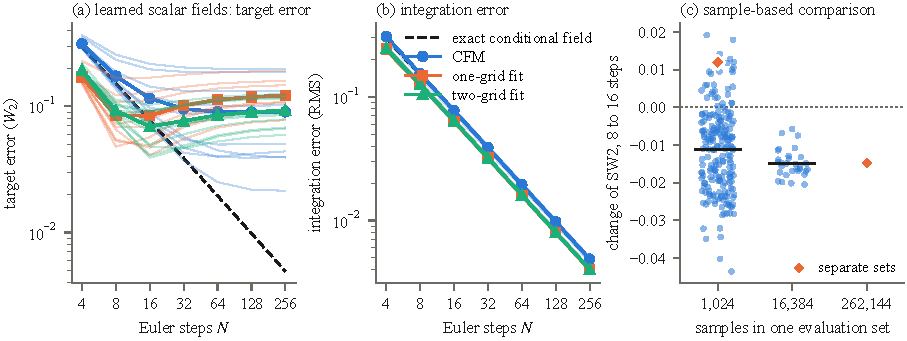
\includegraphics[width=\textwidth]{figures/fig2_learned.pdf}
\caption{Learned fields. (a) Target error of learned scalar fields in
the population $W_2$ distance. Thin lines are the ten seeds of each
objective, and lines with markers are their means. Fields that are
fitted at 8 steps, or at 8 and 16 steps, have their smallest target
error near those step counts. (b) The integration error of the same
fields decreases at first order for all objectives. The legend is for
panels (a) and (b). (c) Change of the
empirical sliced Wasserstein distance (SW2) from 8 to 16 steps,
averaged over six fitted two-dimensional fields. Positive values show
increases. Each dot is one evaluation set. The lines give the means
for each set size, and the diamonds give the values for the separate
sets of 1,024 and 262,144 samples.}
\label{fig:learned}
\end{figure*}

\subsection{Exact Population Computations}
\label{sec:population-example}
Fig.~\ref{fig:rates}(b) shows the scalar Gaussian path of
Section~\ref{sec:sharpness}. For the secant field, $N(E_c+E_f)$ is
$0.666$ at $N=8$ and $0.6428$ at $N=4096$. The limit
in~\eqref{eq:sharp-main} is $(2+\pi)/8\approx0.6427$. The exact
generator has the limit $3(2+\pi)/8$.

Fig.~\ref{fig:rates}(c) shows the two other regimes. For first order,
take the path~\eqref{eq:independent} in dimension three. The first
target coordinate is an equal mixture of Gaussians with means $\pm1.5$
and standard deviation $0.5$. The other two coordinates are centered
Gaussians with the same standard deviation. We compare two exact
generators. The first is the conditional field. The second uses the
skew field of Section~\ref{sec:odd} in the Gaussian plane, which makes
Euler exact in that plane. Theorem~\ref{thm:odd-transfer} gives a lower
bound $c/N$ for both. With the conditional field, $E_c+E_f$ decreases
from $0.292$ at $N=8$ to $0.0096$ at $N=256$. With the skew field, it
decreases from $0.228$ to $0.0074$. The observed orders between $N=128$
and $N=256$ are $0.997$ and $0.998$. The skew field removes the error in
the plane, and the error in the mixture coordinate stays at first order.

For second order, take $d=2$ and the rotation field
$u(t,x)=\tanh(t)x+Jx$, where $J$ is the rotation by a quarter turn. It
generates $p_t=\mathcal N(0,\cosh^2(t)I)$. Its acceleration $2\tanh(t)Jx$ moves particles around circles.
Rotation leaves the Gaussian unchanged, so the acceleration preserves
each $p_t$. Theorem~\ref{thm:characterization} predicts second order.
The scaled error $N^2(E_c+E_f)$ is $0.68$ at $N=8$ and $0.79$ at $N=256$.

\subsection{Learned Scalar Fields With Population Errors}
\label{sec:scalar-learned}
In one dimension, $W_2$ pairs points with the same cumulative
probability. For example, it pairs the two medians. We estimate
population errors by quadrature, which approximates an integral with
a weighted sum. The target is the mixture
coordinate above with the path~\eqref{eq:independent}, so
Theorem~\ref{thm:odd-transfer} applies with $d=1$.

We train networks with two hidden layers of 48 tanh units on three
objectives, with ten random seeds per objective. \emph{CFM} uses the conditional flow
matching loss~\citep{lipman2023flow}. The \emph{one-grid fit} adds a
loss for agreement with the target path in a run of eight Euler steps.
The loss uses the times $1/4$, $1/2$, $3/4$, and $1$. The \emph{two-grid fit} adds
this loss for runs of eight and of sixteen steps. The added loss is the
squared $W_2$ distance between sorted batches. The step size is not an
input of the networks. Training uses
Adam~\citep{kingma2015adam}, and all settings were fixed before the
evaluation.

We report three quantities. The \emph{target error} at $N$ steps is the
largest $W_2$ distance to the target path at the four times. The
\emph{integration error} is the largest root mean squared (RMS) distance
to the exact flow of the field from the same start points. The
\emph{model bias} is estimated as the largest $W_2$ distance between
a reference solution of the flow and the target at 64 times. The errors $E_c$ and $E_f$
of~\eqref{eq:errors} use all nodes of the coarse grid. Supplementary
Table~\ref{tab:scalar-models} gives them for $N=8$.

\begin{table}[t]
\caption{Learned scalar fields: means over ten seeds of population
errors at $N$ Euler steps. The exact field is the conditional velocity,
without training. Supplementary Table~\ref{tab:scalar-models} gives each
field.}
\label{tab:scalar}
\centering
\footnotesize
\begin{tabular}{@{}l@{\hspace{5pt}}c@{\hspace{5pt}}c@{\hspace{5pt}}c@{\hspace{5pt}}c@{\hspace{7pt}}c@{\hspace{7pt}}c@{\hspace{5pt}}c@{}}
\toprule
 & \multicolumn{4}{c}{Target error} & Model & \multicolumn{2}{c@{}}{Integration error}\\
\cmidrule(lr){2-5}\cmidrule(l){7-8}
Field & $N{=}8$ & $16$ & $64$ & $256$ & bias & $N{=}8$ & $256$\\
\midrule
Exact field & 0.151 & 0.077 & 0.020 & 0.005 & 0.000 & 0.151 & 0.005\\
CFM & 0.174 & 0.115 & 0.090 & 0.090 & 0.091 & 0.153 & 0.005\\
One-grid fit & 0.085 & 0.084 & 0.113 & 0.122 & 0.125 & 0.125 & 0.004\\
Two-grid fit & 0.092 & 0.069 & 0.085 & 0.093 & 0.096 & 0.126 & 0.004\\
\bottomrule
\end{tabular}

\end{table}

Table~\ref{tab:scalar} and Fig.~\ref{fig:learned}(a,b) give the results.
The integration error decreases at about first order for all objectives. The
target error does not. For the CFM fields, it decreases from
\ScalarCfmEight{} at 8 steps to \ScalarCfmLarge{} at 256 steps. Their
mean model bias is \ScalarCfmBias{}, with values between
\ScalarCfmBiasMin{} and \ScalarCfmBiasMax{} for the ten seeds. The one-grid fit decreases the mean target error
at 8 steps to \ScalarOneEight{}. For these fields the target error is
larger at 64 steps and at 256 steps than at 8 steps, for all ten seeds.
The exact two-sided Wilcoxon signed-rank test gives
$p=\ScalarOneWilcoxonSixtyFour$ for each of the two comparisons. The change from 8
to 16 steps has no consistent direction: the target error increases for
\ScalarOneIncreaseSixteen{} of the ten seeds ($p=\ScalarOneWilcoxonSixteen$).
Between 8 and 256 steps the mean target error increases by a factor of
\ScalarOneGridFactor{}, while the mean integration error decreases from
\ScalarOneOwnEight{} to \ScalarOneOwnLarge{}. For the two-grid fields,
the target error is smallest at 16 steps for \ScalarTwoArgminSixteen{}
of the ten seeds. For all 20 fitted fields, the target error is larger
at 64 steps and at 256 steps than at 16 steps. The test gives
$p=\ScalarTwoFromSixteenWilcoxonSixtyFour$ for each objective and each
comparison. For all ten CFM fields, the target error is smaller at 64
and at 256 steps than at 16 steps.

For a fixed field, the target error at the four evaluation times
approaches the bias of the exact flow at those times. A coarse run can
offset part of this bias. In the fitted fields, finer runs approach
the exact flow as their error against the target increases. These
comparisons hold the field fixed. Theorem~\ref{thm:characterization}
instead concerns the best error over a class of fields.

\subsection{Sample-Based Comparisons in Two and Eight Dimensions}
\label{sec:sample-based}
In higher dimension, the target error is estimated from samples. We
test how reliable a comparison of two step counts then is. We train 18
tanh networks on mixtures of four Gaussians in dimensions two and
eight, with three seeds for each of the objectives CFM, one-grid fit,
and two-grid fit. Here the added losses compare averages of random
Fourier features~\citep{gretton2012kernel}, and the two-grid fit also
has a term for agreement between the two runs (Supplementary
Section~\ref{app:experiments}). We project the samples onto a line in each of 128 fixed directions
and compute the scalar $W_2$. The root mean square over directions is
the empirical sliced Wasserstein distance (SW2)~\citep{bonneel2015sliced}.
We report its maximum over five times. We call the one-grid and
two-grid fields the \emph{fitted fields}.

On the 1,024-sample evaluation set, all six fitted
two-dimensional fields have a larger SW2 at 16 steps than at 8 steps.
On the independent set of 262,144 samples, all nine fields have
a smaller SW2 at 16 steps (Supplementary Tables~\ref{tab:small-bank}
and~\ref{tab:large-bank}). To measure how often the direction changes, we evaluated the same
fields on \VarSetCount{} sets of two sizes
(Fig.~\ref{fig:learned}(c), Supplementary
Section~\ref{app:set-variability}). Take first the sets of 1,024
samples. The change for a fitted field has a standard deviation of
\VarSmallChangeSd{} between sets and a mean of $\VarSmallChangeMean$.
These values are averages over the six fields. SW2 increases in
\VarSmallFractionMin{}\% to \VarSmallFractionMax{}\% of the
\VarSmallSets{} sets, as a function of the field. All six fields show
an increase together in \VarSmallAllSix{}\% of the sets, as they do in the separate 1,024-sample set. With 16,384 samples,
SW2 increases in at most \VarMediumFractionMax{}\% of the
\VarMediumSets{} sets per field. On the 262,144-sample set, it
decreases for all six. A single small set can give the opposite
direction to the larger set for these fields. For the CFM fields, SW2
decreases from 8 to 16 steps in all sets.

The change from 8 to 64 steps differs between the fields. With 16,384
samples, SW2 is larger at 64 steps than at 8 steps in
\VarMediumLongOneA{}\%, \VarMediumLongOneB{}\%, and
\VarMediumLongOneC{}\% of the sets for the three one-grid fields. The
values for the three two-grid fields are \VarMediumLongTwoA{}\%,
\VarMediumLongTwoB{}\%, and \VarMediumLongTwoC{}\%. For the one-grid field with the value
\VarMediumLongOneA{}\%, simultaneous
confidence intervals for a finite set of bounded test
functions~\citep{hoeffding1963probability,maurer2009bernstein,muller1997integral}
also establish the increase for that set of functions (Supplementary
Sections~\ref{app:statistical} and~\ref{app:large-bank-timing}). The 8-to-64 increase therefore depends on the field and the
measurement in this two-dimensional example.
